\chapter{Progettazione e realizzazione}\label{capitolo:progettazione_realizzazione}
\markboth{Progettazione e realizzazione}{}
Questo capitolo è dedicato alla comprensione e descrizione delle fasi di progettazione e realizzazione di \visualnetkit{}. Si mostretà in maniera dettagliata la nuova struttura dei \plugin{} accennata nel precedente capitolo, e successivamente verrà mostrato il resto del sistema analizzando i singoli moduli che lo compongono.

\begin{figure}[!htb]
	\centering
	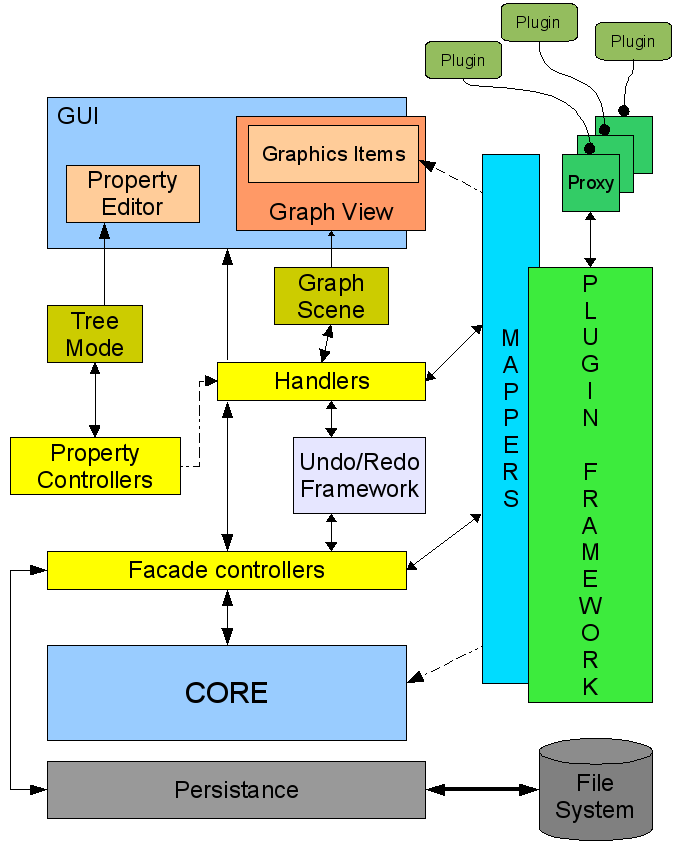
\includegraphics[width=8cm]{images/diagramma_componenti_vnetkit.png}
	\caption{Diagramma dei componenti di \visualnetkit{}}
	\label{figura:vn_componenti}
\end{figure}

In questa introduzione vogliamo subito dare al lettore un quadro generale (figura \ref{figura:vn_componenti}) della composizione architetturale nello stato attuale di \visualnetkit{}, in modo da rendere più facile la localizzazione degli elementi durante la loro trattazione.

\section{Architettura modulare basata su \plugin{}}
Come primo argomento vogliamo concentrarci sulla trattazione della struttura modulare di \visualnetkit{}, che rappresenta anche il suo punto di forza in ambito di flessibilità ed estendibilità. 

Può essere auspicabile che un software pur uso in ambito scientifico sia in possesso di funzionalità opzionali, vale a dire funzionalità che possono essere aggiunte o rimosse nel corso di una simulazione senza grossi ostacoli. Per esempio, si pensi a quanto può essere utile ad un progettista osservare il comportamento di una rete con o senza un tederminato servizio (ad esempio \emph{IPv6}) sulle macchine di cui è composta, o per uno studente quanto risulti comprensibile studiare una topologia di rete malleabile che si presta a tutti i possibili test che egli vuol effettuare.

L'utilizzo di un'architettura basata su \plugin{} dona grande flessibilità all'intero sistema ed in particolare agli utenti finali.

\subsubsection{Perché un sistema basato su \plugin{}?}
Durante le prime iterazioni e le prime fasi di testing emersero alcuni fattori di alto rischio; l'architettura era stata concepita e realizzata basandosi fortemente sul concetto che tutti i requisitivi dovevano essere assemblati staticamente nell'applicazione (come accade nei vari ambienti di configurazioni descritti nella sezione \ref{subsection:ccrc}).

Questa scelta prevedeva una lunghissima fase di sviluppo ed una continua ricerca e specifica dei requisiti e dei casi d'uso che avrebbero potuto destabilizzare l'intero sistema. Inoltre adottando questa tecnica non si sarebbe mai riusciti ad offrire una totale elasticità, ma piuttosto si sarebbe dovuto scendere a compromessi su cosa implementare e cosa no.

Analizzando meglio gli obiettivi si è giusti alla conclusione che l'unica strada percorribile fosse quella che prevedeva la trasformazione dell'architettura in una modularizzata. Il core del sistema (senza alcun \plugin{} attivo) avrebbe offerto all'utente solamente la possibilità di creare una rete a livello topologico, priva quindi di caratteristiche proprie.

Questa nuova tecnica avrebbe da un lato offerto una sicura controllabilità dei fattori di rischio, restringendoli alla re-ingegnerizzazione del sistema per renderlo modulare, dall'altro avrebbe reso \visualnetkit{} estremamente scalabile e flessibile e gli avrebbe conferito una connotazione del tutto unica nel suo genere.

\subsection{Interazione tra sistema e \plugin{}}
Quando si sviluppa un'applicazione che si basa fortemente su \plugin{} la cosa più importante è definire i confini dell'uno e dell'altro sistema. In poche parole ambiente e moduli devono essere ben descritti per non imbattersi in fenomei di sovrapposizione; questi due mondi devono cooperare, ma non devono intralciarsi né tantomeno svolgere le stesse mansioni.

Dopo un'attenta ed accurata fase di studio si è arrivati a definire la linea di demarcazione tra il sistema e le estensioni. I vari \plugin{} possono essere attivati sugli elementi di base del sistema offrendo una sorta di caratterizzazione più specifica. Su di un elemento possono essere attivi contemporaneamente più \plugin{} che di fatto donano una definizione ben precisa all'elemento. Se per esempio su un host noi attiviamo \plugin{} quali DNS e HTTP, balza subito all'occhio il tipo di quell'oggetto; abbiamo semplicemente di fronte una macchina virtuale che offre un servizio di DNS e che allo stesso tempo è un server Web di qualche tipo.

Andiamo ora a descrivere in dettaglio la struttura del sotto sistema che permette ai moduli di colloquiare con il core dell'applicazione e la definizione delle varie interfaccie - figura \ref{figura:uml_plugin_framework}.

\begin{figure}[!htb]
	\centering
	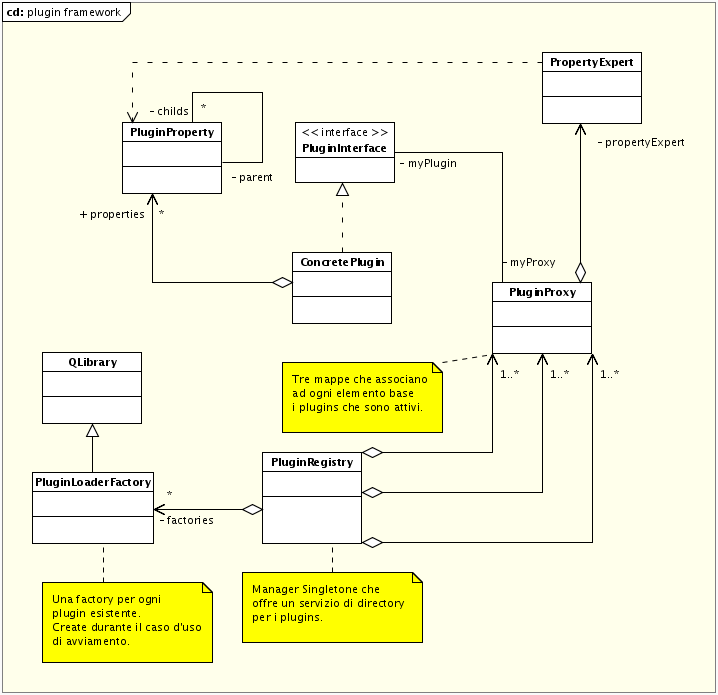
\includegraphics[width=12cm]{images/plugin_framework_uml.png}
	\caption{Diagramma delle classi del sotto sistema di gestione dei \plugin{}.}
	\label{figura:uml_plugin_framework}
\end{figure}



\section{Elementi architetturali}

\subsection{L'interfaccia utente}


\subsection{Gli handlers}

\subsection{Property controllers}

\subsection{Undo Framework}

\subsection{Elementi del dominio}

\subsection{L'accesso al \fs{}}

\subsection{I mappers}

\section{La gestione avanzata delle properties}
\subsection{Properties di base}
\subsection{Properties dei \plugin{}}

\section{Strumenti di supporto allo sviluppo}
\subsection{Il framework \qt{}}
\subsection{Altri strumenti secondari}
